\chapter{Tools and techniques for energy measurement}


The recent scientific applications have to process and store
considerable volumes of data. It is expected that the volume of
data will increase considerably in the future, as technology improvements and
requirements increase. This fact increases considerably
the costs with energy in a HTC system. Thus, energy consumption has
become a major concern amongst the scientific community.

It is critical to understand how energy is used by the HTC systems and its components, in order to develop solutions for improving energy efficiency in HTC. The learnings, techniques and tools can be further implemented in non-HTC systems whith the same results.

This chapter outlines and describes tools and techniques for measuring energy consumption in any machine. Our main goal is to use these tools and techniques to study energy efficiency of HTC systems, more specificcally systems running on top of x86 and ARM architectures. The tools and techniques described in this chapter were used widely during the study of energy efficiency comparison described in the following chapters. 


The results of this section were publish in the conference proceedings of the 16th International workshop on Advanced Computing and Analysis Techniques in physics research (ACAT'2014). The article was called \textit{Techniques and tools for measuring energy efficiency of scientific software applications} \cite{ACAT} and can be found on Appendix A, at the end of this document. 

\section{The big picture}

%granularities
During this study, we will consider two different granularities at which is possible to measure the energy consumption of a computing system. The two granularities are coarse and fine granularity and they differ on the type of system components that are taken into consideration when measuring energy consumption.

The coarser granularity takes into account the behavior of the whole node. This is usually investigated when
engineering and optimizing computing centers. Alternatively, a more detailed approach is to
look into the components which make up the active parts of a
node, in particular the CPU and its memory subsystem since these
are responsible for a sizeable fraction of the consumed power.
They are also the place where the largest gains in terms of efficiency 
can be obtained through optimizations in the software \cite{ACAT}.

\subsection*{Coarse grain or external measurements}
As stated by \cite{ACAT}, If one is simply interested in the coarse power consumption by node,
external probing devices can be used: monitoring interfaces
of the rack power distribution units, plugin meters and non-invasive
clamp meters (allowing measurement of the
current pulled by the system by induction without making physical
contact with it). They differ mostly in terms of flexibility.
Their accuracy is typically a few percent for power, whereas their time
resolution is in the order of seconds. This features are enough
to optimize electrical layout of the datacenters or to provide a
baseline for more detailed studies.

\subsection*{Fine grain or internal measurements}
A alternative approach takes into account the internal structure of a
computing element of an HTC system, as shown in figure 
~\ref{fig:power-consumption-model}. Nowadays, almost all board manufacturer
provides on-board chips which monitor energy consumption of
different components of the system. These
allow energy measurements of fine grained detail, as it is possible
to individually monitor energy consumption of components such as
the CPU, its memory subsystem, and others. An example of this chip
monitors is the Texas Instruments TI INA231~\cite{TIINA231} current-churn
and power monitor which is found on the ARMv7 developer board which
we used for our studies. It is quite common in the industry.e
Compared to external methods, these on-board components provide
high accuracy and reasonably high precision measurements (millisecond
level).

\begin{figure}[tbp]
\centering
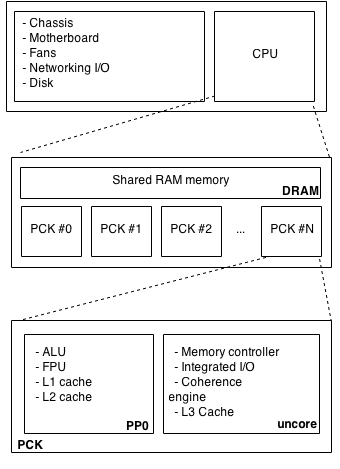
\includegraphics[width=75mm]{img/energy_model.png}
\caption{Components that contribute for power consumption in HPC. Taken from \cite{ACAT}}
\label{fig:power-consumption-model}
\end{figure}

\section{Tools for measuring energy consumption}

\subsection*{Internal tools}

\subsubsection*{Running Average Power Limit}
%internal tools
%RAPL
Recent Intel boards provide a powerful way to measure fine grained energy consumption of their CPUs with the Running Average Power Limit (RAPL) technology. RAPL has been included on the SoC from the factory since the Sandy Bridge family of processors.

Contrary to other solutions (such as TI INA231, for example), which are implemented as discrete
chips, RAPL is embedded as part of the CPU package itself and
provides information on the CPUs own subsystems. In particular RAPL
provides data for three different domains: \textbf{package} (pck),
which measures energy consumed by the system's sockets, \textbf{power
plane 0} (pp0), which measures energy consumed by the CPU core(s),
and \textbf{dram}, which accounts for the sum of energy consumed
by memory in a given socket, therefore excluding the on-core
caches~\cite{INTELMAN}. As for the discrete components case, the
timing resolution of measurements is in the millisecond range~\cite{RAPL1}.
This is fine enough to allow exploiting such data to build an energy
consumption sampling profiler for applications, similar to how performance
sampling profilers work (see section~\ref{sec:sampling}).
Finally, in addition to power
monitoring of the sockets, RAPL can limit the power consumed by the
different domains. This feature, usually referred as power capping,
allows the user to define the average power consumption limit of a
domain in a defined time window and allows more accurate independent
measurements of the non limited components.

\subsubsection*{TI INA 231}
There are chips that provide similar power monitoring capabilities than RAPL, but for any architecture and technology. An example is the Texas Instrument (TI) INA231 \cite{TIINA231}. The TI INA231 is a power monitor that reports current, voltage and power consumption of CPU, DRAM and cores of the SoC which is attached. Some vendors include the TI INA231 in their boards from origin, relying on an external technology to provide the same capabilities as RAPL monitoring.

Similarly to RAPL, the sampling resolution is high (at the sampling rate of microseconds) and the error is relatively low. On the other hand, the TI INA231 does not have capping capanilities.


\subsection*{External tools}

There are different techniques and tools to measure the power consumed by the whole system ~\ref{fig:power-consumption-model}. Usually when the system is part of a server rack, the rack itself offers an API to sample the power consumed by each of the systems and overall rack power consumed. For simpler systems, it is recommended to use either power sockets with power meters or an external power meter. 

The resolution and errors of external tools vary according to their nature. The resolution can range from microseconds - when the sampling is done digitally - to seconds - when the sampling is done by a person. It is recommended to use API and digital based external tools in order to achieve the best resolution and error possible. 



\section*{Conclusion}
There are many different methodologies and tools to measure energy consumption of computing systems. The differences between the existent options range from granularity, accessibility, error and resolution and also from hardware or software approaches. The decision for which tools and techniques should be relied upon for the measurements is important when conducting research on energy efficiency. The decision is directly dependent on the goals of the experiment and the availability of the tools according to the technology to be used. 

Most of the techiques and tools outlined in this section were used in our experiments and are further discussed in the Experiments and Analysis chapters. In addition, the original paper which dwelves into the techniques and tools in more detail and was published at the ACAT'2014 conference proceding is attached as Appendix A.